\chapter{Analyser}\label{Analyser}

\section{Brugerundersøgelse}
Der er foretaget to slags brugerundersøgelse, en kvantitativ med potentielle patienter og to kvalitative interviews med en overlæge og en specialeansvarlig radiograf. Dette er medtaget for at belyse, hvordan vil en automatiseret ultralydsscanner til screening for brystkræft modtages af patienter og personale. 

\subsection{Spørgeskemaundersøgelse}
Undersøgelsen bestod af et kvalitativt spørgeskema med tre spørgsmål, omhandlende scanning med en automatiseret robotarm fremfor en læge, samt hvilke problemstillinger og fordele respondenterne ser ved en automatiseret ultralydsscanner. Spørgeskemaundersøgelsen blev lavet før projektet var færdigdefineret og derfor falder den lidt ved siden af projektet, den er dog stadig medtaget i projektet, fordi den kan give et billede af, hvordan patienter vil tage imod Automatisk Ultralydsscanner.  

Der var i alt 72 respondenter på spørgeskemaet, hvor størstedelen, 87,5\%, af respondenterne var positive for at blive scannet af robotarmen hvis kvaliteten og sikkerhed er på højde med, hvad den er, når en læge foretager en ultralydsscanningen. De sidste 12,5\% som var negative for automatisk scanning med en robotarmen frygter, at robotarmen vil lave fejl, det bliver upersonligt, og at det vil give en fornemmelse af, at lægen har berøringsangst for patienterne. 
De problemstillinger respondenterne ser ved automatiserede ultralydsscanninger, var at robottens følsomhed mangler, og det måske kan gøre undersøgelsen ubehagelig og utryg for patienten. Samtidig nævner flere bekymringer for robottens evne til at scanne forskellige kropstyper. Fordelene, som respondenterne så ved automatiserede ultralydsscanninger var, at robotten måske kan give økonomisk mening med kortere ventetider og spare tid og dermed frigøre ressourcer i form af personale til andre opgaver. Flere af respondenter mente, at en robotarm kan reproducere scanningerne og er derfor ikke afhængig af, hvor god lægen er. Den yngre del af respondenterne nævner ergonomiske fordele for lægen, mindre blufærdighed og langdistance-undersøgelser, som andre fordele. 

Se bilag \ref{Sporgeskemaundersogelse} Spørgeskemaundersøgelse, for hele spørgeskemaundersøgelsen. 

\subsection{Besøg og interview på Aarhus Universitetshospital, Tage-Hansens Gade} 
Aarhus Universitetshospital, Tage-Hansens Gade blev kontaktet til inspiration og belysning af den daglige praksis på en røntgen- og skanningsafdeling, samt undersøgelse af sundhedsfagliges meninger om Automatisk Ultralydsscanner. Radiograf Tine Bisgaard indvilgede i at vise rundt på afdelingen samt svare på spørgsmål om afdelingens dagligdagen. På daværende tidspunkt var Automatisk Ultralydsscanner ikke afgrænset til at kunne indgå i som supplement til mammografi i screeningspakken. 

Tine Bisgaard vurderede mammografi af begge bryster til at tage 5 minutter, mens en ultralydsscanning blev vurderet til at tage omkring 10 minutter, afhængigt af radiologens rutine. Tine Bisgaard mente ikke, at det vil være et problem at benytte en Automatisk Ultralydsscanner til at udføre scanninger, hvis man blot informerer patienterne. Hun ser dog en ulempe ved at lade en radiograf lave scanningerne idet, patienten ikke kan få svar med det samme, hvilket de normalt får når en radiolog udføre ultralydsscanningen. Tine Bisgaard nævnte yderligere en ulempe, hun frygter at det vil tage længere tid at foretage scanningen og derefter få en radiolog til at vurdere billederne.

Fordelene, Tine Bisgaard ser ved en Automatisk Ultralydsscanner er, at man på afdelingerne er nødt til at tænke i nye baner i forhold til manglen på radiologer i Danmark. Derfor mener hun, at det vil være smart, hvis radiograferne kunne udføre en del af arbejdet med ultralyd for at spare tid og penge. Tine Bisgaard og en unavngiven kollega på afdelingen foreslår, at proceduren kan gøres simpel, dvs. gøre svare kvantitative f.eks. mål, ja/nej. Det ser hun som måden en radiograf vil kunne styre en Automatisk Ultralydsscanner. På baggrund af interviewet og rundvisningen på afdelingen, blev der i projektet fokus på, hvordan en procedure for Automatisk Ultralydsscanner kukke gøre simpel, og om substitueringen af radiologer med radiografer ville kunne være en økonomisk gevinst. Derudover blev det besluttet at Automatisk Ultralydsscanner max måtte være 10 minutter om at udføre 3D scanning og efterfølgende ultralydsscanning. 

Se bilag \ref{Tine} Interview med afdelingsradiograf Tine Bisgaard, for hele interviewet. 

\subsection{Interview med radiolog og ultralydsekspert}
Der blev foretaget et telefonisk interview og efterfølgende et opfølgende møde med radiolog og ultralydsekspert, Lars Bolvig. Interviewet blev lavet for at undersøge proceduren ved ultralydsscanninger af brystet. Der var på forhånd defineret nogle spørgsmål angående lokalisering af knuder, hastigheder og tiden en læge typisk vil bruge på en ultralydsscanning af brystet og lokalisering af knuder. Ifølge Lars Bolvig vil en læge kunne lokalisere en knude i brystet på 2-3 minutter, mens hastigheden, der scannes med, er meget operatørafhængig. Lars Bolvigs forslag til hvor det vil give mening at implementere Automatisk Ultralydsscanner var til supplement til mammografi. Det vil sige, at Automatisk Ultralydsscanner vil kunne give mening at implementere som en udbyggelse af screeningsproceduren med mammografi, som anvendes i dag. Dette kunne give mening fordi, at man med en efterfølgende ultralydsscanning, efter en mammografiundersøgelse, vil kunne opdage flere kræfttilfælde. 

Lars Bolvig fortalte, at ved ultralydsscanning af brystet, føres ultralydsproben i en sinus-lignende kurve hen over brystet. Probens bane skal overlap og man tager et bryst af gangen. Det skal sikres, at ultralydsproben starter og slutter uden for brystvævet, for at sikre at at hele brystet er scannet. Bevægelsesmønsteret er illustreret i Figur \ref{Probensbevagelse} nedenfor. 

\begin{figure}[H]
    \centering
    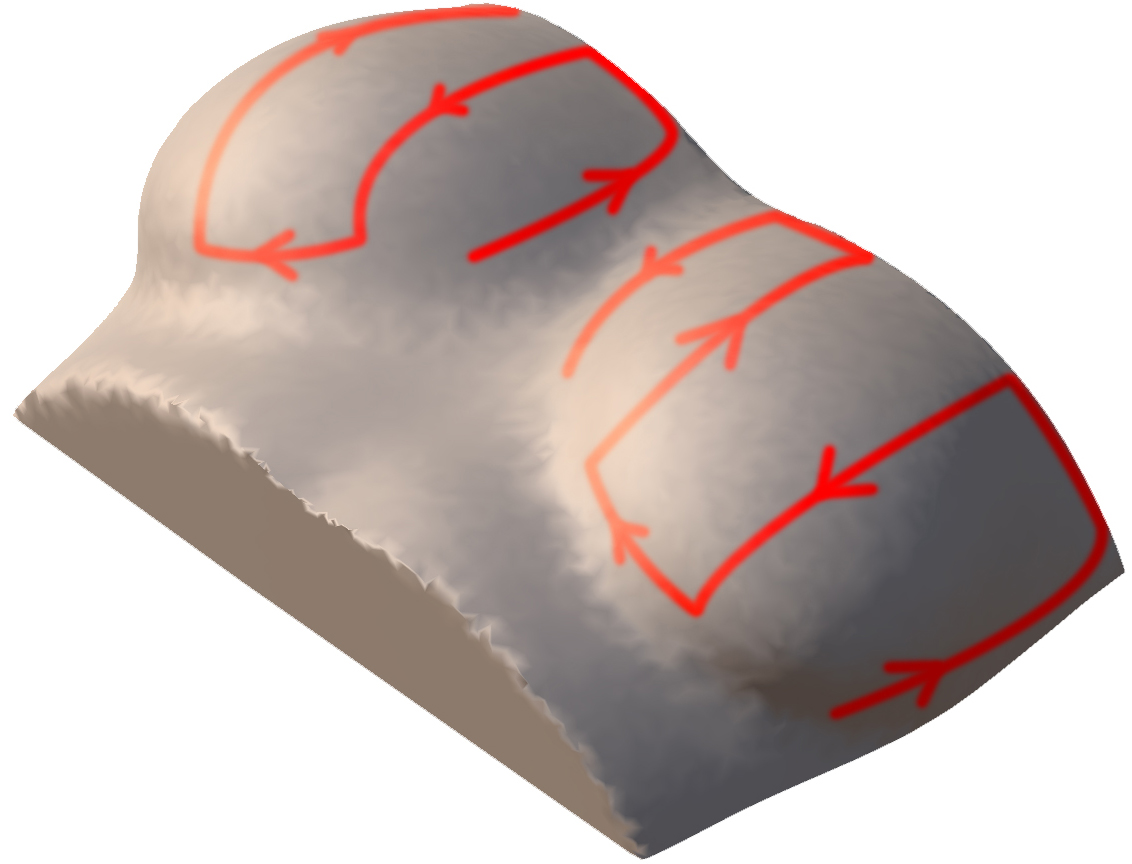
\includegraphics[width=0.75\textwidth]{figurer/d/probebevagelse}
    \caption{Det specifikke bevægelsesmønster ved scanning}
    \label{Probensbevagelse}
\end{figure}

Lars Bolvig tilføjede også, at Automatisk Ultralydsscanner skal kunne betjenes af radiografer. Så Automatisk Ultralydsscanner skal fungerer ved, at radiografen tager videoclipsne fra ultralydsscanningen og sender dem til radiologen, som bestemmer videre behandlingsforløb.

Se bilag \ref{Telefoninterview} Telefoninterviewet med radiolog Lars Bolvig. 

\section{Økonomisk og omkostningseffektiv analyse}
Formålet med denne analyse er at belyse det økonomiske perspektiv, ved at mammografiscreeningsprogrammet blev udvidet til at inkludere ultralydsscanninger. Den økonomiske analyse er udført ved at lave et overslag over forskellen på udgifterne, hvis en radiolog skulle udføre ultralydsscanningerne, versus indførsel og implementering af Automatisk Ultralydsscanner, hvor en radiograf udføre ultralydsscanningerne. Til at belyse konsekvenserne ved at udvide screeningsprogrammet er der søgt nationale og internationale litteratur om emnet. 

\subsection{Økonomiske konsekvenser ved udvidelse af screeningsprogrammet} 
Den økonomiske analyse er et overslag med udgangspunkt i en breakeven analyse. Efter interview med radiograf Tine Bisgaard og radiolog Lars Bolvig, blev det sandsynliggjort, at radiografer kan betjene Automatisk Ultralydsscanner, hvorefter videoclip fra ultralydsscanningen gennemses af en radiolog, samme procedure, som ved mammografi. 
Radiologer bruger i dag tid på at transportere sig til og fra scanningsstedet, når der skal scannes på patienter. Transporttid er derfor en vigtig variabel i breakeven analysen. Breakeven analysen tager udgangspunkt i, hvor mange ressourcer der kan flyttes fra en radiolog til en radiograf, ift. omkostningen relateret til implementeringen af Automatisk Ultralydsscanner, hvis screeningsprogrammet blev udvidet. 

Det er antaget, at radiologs gennemsnitlig løn er omkring 369 kr./timen, mens en radiografs gennemsnitlige løn er omkring 173 kr./timen \cite{Lon}. De samlede omkostning for anskaffelse af udstyret til opsætning af Automatisk Ultralydsscanner er fundet ved indsamling af priser fra forskellige hjemmesider (Se bilag \ref{Okonomi} Økonomi for flere oplysninger). De samlede faste omkostninger for fuld implementering inkluderer engangsudgifter for opsætning og oplæring af radiografer i anvendelse af Automatisk Ultralydsscanner. Den samlede pris for Automatisk Ultralydsscanner ligger omkring 219.305,64 kroner, de samlede udgifter kan ses i Tabel \ref{FasteOmkostninger}. 

\begin{table}[htb]
\centering
\begin{tabular}{ | l | l | p{1\textwidth} | }
\hline
\textbf{Beskrivelse af udgift} & \textbf{DKK} \\\hline
Engangsudgifter til afskrivning & 201.668,00 \\\hline
Opsætning & 10.759,00 \\\hline
Oplæring af radiografer & 6.768,00 \\\hline
I alt & 219.305,64 \\\hline
\end{tabular}
\caption{Samlede udgifter for Automatisk Ultralydsscanner}
\label{FasteOmkostninger}
\end{table}

Der er for begge scenarier blevet beregnet en pris for én ultralydsscanning. Prisen pr. scanning med Automatisk Ultralydsscanner er nogenlunde konstant, mens den varierer ved scenariet, hvor radiologen foretager ultralydsscanningen, priserne variere grundet forskellige transporttider for radiologen.  
Prisen for én scanning med Automatisk Ultralydsscanner er udregnet ved at antage, at det er en radiograf, der foretager forberedelse, 3D scanning og selve ultralydsscanningen, hvorefter en radiolog vil bruge omkring 10 minutter på at tjekke scanningen igennem for at se, om patienten skal til en yderligere scanning. Prisen for dette er beregnet til 110,64 kroner. 

Prisen for én ultralydsscanning ved scenariet, hvor en radiolog foretager ultralydsscaningen, er udregnet ved at antage, at det er en radiolog, der foretager både forberedelse, ultralydsscreening og transporttid på komme frem og tilbage til scanningsstedet. Hvis transport for radiologen er under fire minutter, er scenariet med Automatisk Ultralydsscanner dyrest. Automatisk Ultralydsscanner er derimod billigere hvis transporttid er over 4 minutter. Tabel \ref{Breakeven} beskriver transportminutter, pris for én ultralydsscanning udført af radiolog, og total antal scanninger udført, før før Automatisk Ultralydsscanner er betalt hjem. 

\begin{table}[htb]
\centering
\begin{tabular}{ | c | c | c | p{0.49\textwidth} | }
\hline
\textbf{Transporttid (min)} & \textbf{Pris per scanning (DKK)} & \textbf{Antal screeninger} \\\hline
5 & 116,89 & 35.052,51 \\\hline
8 & 135,34 & 8.873,09\\\hline
10 & 147,64 & 5.923,66\\\hline
15 & 178,39 & 3.235,19 \\\hline
20 & 209,14 & 2.225,25\\\hline
30 & 270,64 & 1.369,94\\\hline
45 & 362,89 & 868,95 \\\hline
60 & 455,14 & 636,26 \\\hline
\end{tabular}
\caption{Breakeven analyse for antal transportminutter}
\label{Breakeven}
\end{table}

Analysen er et overslag og ikke en nøje udført business case, da alle udregningerne er skøn. Analysen ville fremstå bedre, hvis der havde medvirket flere radiologer og radiografer til estimering af tider på ultralydsscanninger. Det er generelt forsøgt at prissætte udgifterne forbundet med indførslen af Automatisk Ultralydsscanner relativt højt for at undgå for mange uforudsete omkostninger. Hvis et hospital vil købe udstyret, vil priserne for opsætning måske være lavere, hvis man laver en indkøbsaftale. Beregningerne har ikke taget højde for, at radiologen udfører flere ultralydsscanninger for en transporttid. Transporttid må derfor ses som et gennemsnit pr. patient. 

Der bliver i Danmark udført omkring 270.000 mammografiundersøgelser om året, som en del af screeningsprogrammet \ref{esundhed}. Det betyder, at Automatisk Ultralydsscanner med en pris på 110,64 kroner pr. ultralydsscanning vil øge udgifterne til screeningsprogrammet med omkring 30 mio. kroner om året. yderligere vil der være ekstra omkostninger ved vedligeholdelse på Automatisk Ultralydsscanner.  

\subsection{Konsekvenser af udvidelse af screeningsprogram} 
Til belysning af konsekvenser

Ved at udvide screeningsprogrammet, vil der ifølge studiet 

"Sensitivity and specificity of mammography and adjunctive ultrasonography to screen for breast cancer in the Japan Strategic Anti-cancer Randomized Trial (J-START): a randomised controlled trial (2016)” af Ohuchi N. et al 

